%base packages 
\documentclass[11pt]{article}
\usepackage[margin=1in]{geometry}
\usepackage{caption,multirow,etoolbox,color,enumerate,amsmath,dsfont,lscape,tocloft,booktabs,draftwatermark,array,tabularx,graphicx,pdflscape,subcaption}
\usepackage{setspace}
\setlength{\parskip}{0em}
\usepackage[bottom, flushmargin]{footmisc}
\usepackage[T1]{fontenc}
\usepackage[utf8]{inputenc}
\usepackage{lmodern}
\usepackage[english]{babel}
\usepackage[autostyle]{csquotes}
\makeatletter
\makeatother
\usepackage{float}
\SetWatermarkText{}\SetWatermarkLightness{0.85} \SetWatermarkScale{4}
\usepackage{appendix}
\usepackage{authblk}
\usepackage[format=hang,justification=raggedright,singlelinecheck=0,labelsep=period]{caption}
%[format=hang,justification=raggedright,singlelinecheck=0,labelsep=period]
%\usepackage[numbers,sort&compress]{natbib} %Use this set-up for numbered reference lists
\usepackage[authoryear]{natbib} %Use this set-up if you want an un-numbered reference list
%\usepackage{hypernat}

\usepackage[hyperfootnotes=false]{hyperref}
%\usepackage[dvipdfmx,hyperfootnotes=false]{hyperref}
%\usepackage[dvips,hyperfootnotes=false]{hyperref}
\hypersetup{colorlinks=true,linkcolor=blue,anchorcolor=blue,citecolor=blue,filecolor=blue,urlcolor=blue,bookmarksnumbered=true,pdfview=FitB} %
% % %DO NOT PLACE ANY PACKAGES AFTER THE HYPERREF SET UP
\usepackage{titling}

%-----------------------------------------------------------------------%
\begin{document}
\bibliographystyle{mla-good}


\title{Investigating the Inclusive-Performance Tradeoff in Agricultural Cooperatives: Evidence from Nepal\thanks{Copyright 2020 by Scott M. Miller (\href{scottmmiller@ufl.edu}{scottmmiller@ufl.edu}). All rights reserved. Readers may make verbatim copies of this document for non-commercial purposes by any means, provided this copyright notice appears on all such copies.} \thanks{This paper is made possible by the generous support of the American people through the United States Agency for International Development (USAID) and its Feed the Future Innovation Lab for Livestock Systems managed by the University of Florida and the International Livestock Research Institute. The contents are the responsibility of the author and do not necessarily reflect the views of USAID or the United States Government.}}

\author{Scott M. Miller \\ Food and Resource Economics Department \\ University of Florida}
\date{}

\sloppy
\maketitle

\vspace{.5cm}
\begin{center}
\textit{Selected Paper prepared for presentation at the 2020 Agricultural \& Applied Economics Association \\ Annual Meeting in Kansas City, Missouri \\ July 26-28, 2020}  
\end{center}


\vspace{.5cm}

%------------------------------------------%
\begin{abstract}
Is there a tradeoff between inclusive membership and market performance in agricultural cooperatives? The answer to this question is critical for understanding the role that cooperatives play in agricultural development and poverty alleviation. However, studies on this topic have largely focused on membership criteria as the source of inclusion, overlooking the extent to which existing members are included in cooperative activities. This distinction is central to the challenge faced by cooperatives in which including a diverse membership may damage cooperative performance by increasing transaction costs but may also improve performance by pooling a quantity of inputs. In this essay, I use the Oaxaca-Blinder decomposition to further examine this relationship by analyzing i) whether there is a tradeoff between inclusive membership and market performance and ii) whether this tradeoff is explained by differences in observable characteristics or differences in the ability to translate those characteristics into results.
\end{abstract}
%------------------------------------------%

\pagenumbering{gobble}
\clearpage
\renewcommand{\cftsecleader}{\cftdotfill{\cftdotsep}}

\tableofcontents
\clearpage

\doublespacing
\thispagestyle{plain}
\pagenumbering{arabic}
\setcounter{page}{1}

%-----------------------------------------------------------------------%
\section{Introduction} \label{sec:intro}
% Hook
Rural markets in developing countries are often rife with constraints that limit the ability of smallholders to sell in formal markets that provide good prices and generate higher incomes \citep{ashby_investing_nodate,p_kristjanson_notitle_2014}. In these settings, agricultural cooperatives often arise in an effort to increase bargaining power, decrease transaction costs, and help achieve scale economies in marketing \citep{markelova_collective_2010,rondot_agricultural_2001,staal_smallholder_1997,csaki_reaching_2003}. However, evidence suggests that many farmer organizations struggle to generate large and inclusive benefits for their members \citep{bernard_reaching_2009, casaburi_loyalty_2015,poole_review_2010}. The relationship between inclusive membership and market performance has been highlighted as an unresolved conflict in the cooperative literature, where organizations struggle to balance social inclusion with the challenge of coordinating activities among a diverse membership \citep{bernard_reaching_2009,world_bank_world_2008}. 

% Question
Is there a tradeoff between inclusive membership and market performance in agricultural cooperatives? The answer to this question is critical for understanding the role that cooperatives play in agricultural development and poverty alleviation. However, studies on this topic have largely focused on group membership as the source of inclusion, overlooking the extent to which existing members are included in cooperative activities. This distinction is central to the challenge faced by cooperatives in which including a diverse membership may damage cooperative performance by increasing transaction costs \citep{world_bank_world_2008} but may also improve performance by pooling a larger quantity of inputs \citep{aflagah_cheap_2019}. 

% Antecedents
Prior studies argue that cooperatives enforcing performance oriented membership rules are better able to reduce the transaction costs associated with coordination and the management of group activities \citep{world_bank_world_2008}. This issue has received considerable attention in the cooperative literature as these rules tend to exclude the most vulnerable from receiving the benefits associated with cooperative membership, potentially reducing the role of producer organizations in poverty alleviation (\textbf{cite}). Conversely, in the case of coordinating bulk sales of members' output, larger group sizes can improve the bargaining position of the cooperative by increasing the quantity of marketable output. If cooperatives are able to successfully manage the increased coordination challenge associated with group size, large organizations may be able to generate broader benefits \citep{aflagah_cheap_2019}. %CM: You've laid out why membership size may have an ambiguous relationship with cooperative performance. But what about your particular question, i.e. inclusiveness conditional on being a member? If you see the same arguments applying to the extensive (membership size) and intensive (inclusiveness conditional on membership) with regards to cooperative performance, that's fine. But you should make that point. I think it kind of comes down to what the shape of the MC and MB curves are. Does the latter go up with inclusiveness because of bargaining power? Is the former flat, U-shaped, half-U?

% Value Added
In this paper, I expand the definition of inclusive membership to account for the extent to which cooperative members are included in group activities and further examine the inclusiveness-performance tradeoff. Using the \citet{oaxaca_male-female_1973}-\citet{blinder_wage_1973} decomposition, I analyze i) whether there is a tradeoff between inclusive membership and market performance and ii) if so, whether this tradeoff is explained by differences in observable characteristics or differences in the ability to translate those characteristics into results. My population of interest are smallholder goat producers in rural Nepal, all of whom are women and members of agricultural cooperatives. The data used in this study covers 2,856 households across 109 smallholder livestock cooperatives in Nepal. 

I find that cooperatives that include a larger share of illiterate and low asset holding farmers in their membership perform significantly worse than their less inclusive counterparts. While this result is consistent with the inclusive-performance tradeoff, I also find that cooperatives who include a larger share of their members in group activities achieve significantly higher performance than their less inclusive counterparts. Both results are largely driven by differences in returns to the observable characteristics between the most and least inclusive cooperatives. This suggests that both membership criteria and the extent to which existing members are included in activities have a meaningful, but opposite, impact on a cooperative's ability to achieve market performance, and that these results are not explained by differences in observable characteristics between the two groups. %CM: Ok, so you do both dimensions of inclusiveness. That's great. I think my point above still stands though.  


%-----------------------------------------------------------------------%
\section{Background} \label{sec:background}

In Nepal, where 68 percent of the population depends on agriculture for their livelihood %CM: Maybe establish the context in the intro. Otherwise the intro of Heifer in the Background section is a little bit awkward
\citep{international_labor_organization_ilo_2016}, goats are a common source of income and nutrition. This is particularly true in rural areas, where nearly every household owns a least a few goats \citep{upreti_food_2009}. In recent years, urbanization and rising incomes have lead to a higher demand for goat meat, but a poorly functioning value chain has left smallholder producers, most of whom are women, unable to benefit \citep{ashby_investing_nodate,choudhary_pro-poor_2011,gurung_empowering_2015}. Smallholders face high transaction costs, weak bargaining power and a lack of communication infrastructure that limit their ability to access and gain from formal output markets \citep{ashby_investing_nodate,p_kristjanson_notitle_2014}. As a result, domestic production has been unable to keep up with rising demand, leading to higher imports from India and Tibet \citep{heifer_international_nepal_study_2012}.

Many agricultural policy and rural development plans in Nepal have promoted agricultural cooperatives as a means of supporting smallholder producers \citep{agricultural_development_strategy_agricultural_2015}. Non-governmental organizations, including Heifer Project International in Nepal (HPIN), have made recent efforts to strengthen the goat value chain by organizing producer cooperatives. HPIN’s programs give women livestock and extensive training. Beneficiaries are then organized into self-help groups (SHGs) of around 20-30 female members. Once SHGs in a given area are sufficiently organized, they are combined into larger producer cooperatives \citep{janzen_short-term_2018}.

% This follows closely from the VCC Pre-Analysis Plan. In the full dissertation, I will cite this accordingly if that paper moves forward
The majority of goats in Nepal are consumed after sale to a local collector who pools animals from smallholder producers \citep{heifer_international_nepal_study_2012}. For goats that are marketed outside of their original communities, the commercial value chain links producers, local collectors and regional traders to consumers who are primarily located in urban markets \citep{heifer_international_nepal_study_2012}. 


%-----------------------------------------------------------------------%
\section{Data} \label{sec:data}
In this paper I use a cross-sectional dataset covering than 2,856 goat producing households across 108 smallholder livestock cooperatives in Nepal. The cooperatives in this sample are spread across four of five development regions in Nepal, specifically the East, Central, West and Mid-Western Development regions. All cooperatives operate in either the low-land Terai or mid-Hills. Figure (\ref{map}) shows the study area covered in the sample, which includes cooperatives from 24 districts across Nepal. The cooperatives included in the study were selected by HPIN and include all existing livestock marketing cooperatives the organization helped form prior to 2017.

\begin{figure}[!h]
    \caption{Study Area}
    \label{map}
    \noindent \centering 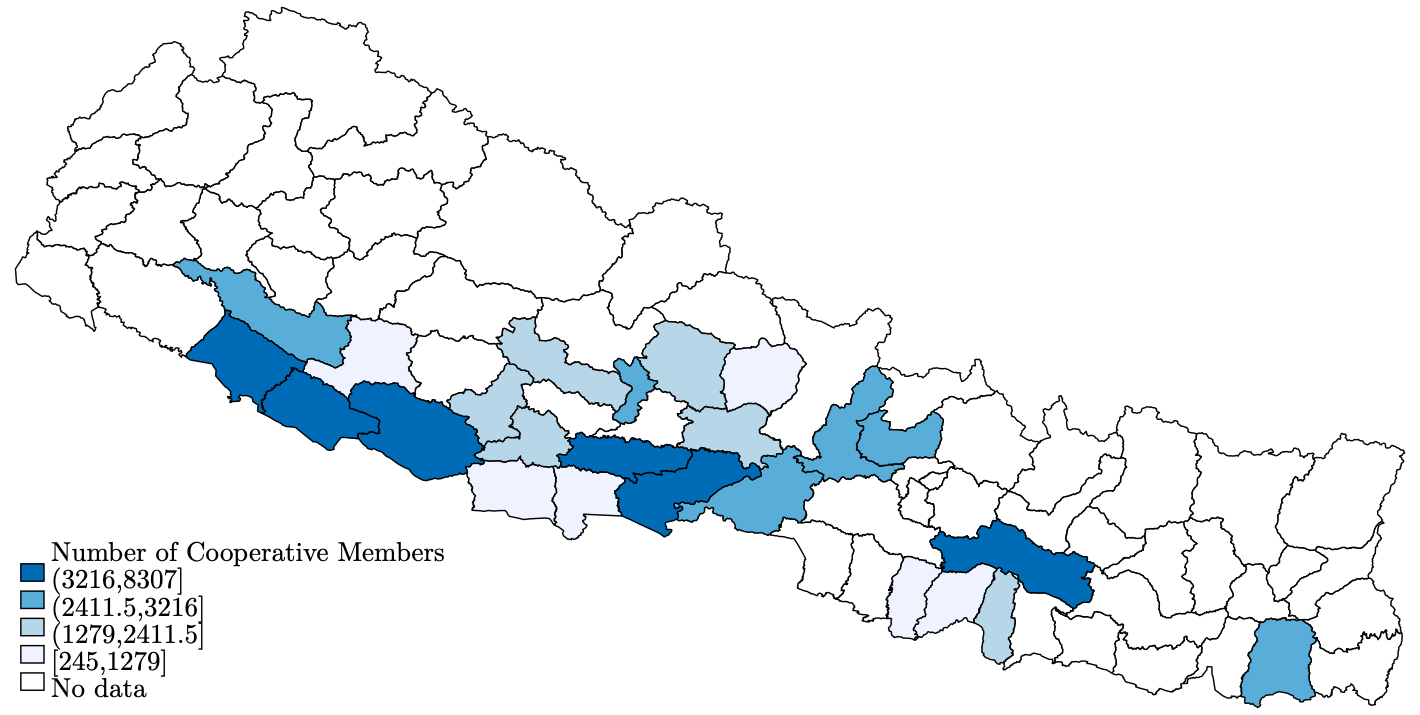
\includegraphics[width=.9\textwidth,trim=4 4 4 4,clip]{StudyMap.png}
\end{figure}

This dataset consists of two separate surveys - one with cooperative leaders and another with general members.  %CM: If this feature of our data is unique in the co-op literature, you could emphasize it a bit more in the intro.
I refer to these surveys as the cooperative leader and household survey, respectively. The cooperative leader survey is comprised of interviews from three officers in each cooperative. To obtain a representative sample for the household survey, HPIN and cooperative leaders generated complete cooperative rosters. From these comprehensive lists, a random sample of 2,856 households across 108 %CM: or 109?
cooperatives was drawn to participate in the household survey. The data were collected from the sample in January 2018 using Android tablets and Open Data Kit.

\singlespacing
% Summary Stats Table
\newcolumntype{Y}{>{\centering\arraybackslash}X}
\begin{table}[!h]
  \centering
  \caption{Summary Statistics}
  \label{table:E1_summary}
  \scalebox{.8}{
  \begin{tabularx}{1.2\linewidth}{l*{7}{Y}}
\hline Cooperative-Level Variables & N & Mean & sd & Min & Max\\
\noalign{\smallskip}\hline \noalign{\smallskip}
Number of members  (count) & 107.00 & 568.64 & 375.77 & 11.00 & 2,600.00\\
Annual revenue (USD) & 108.00 & 3,643.70 & 5,476.12 & 0.00 & 36,785.87\\
Cooperative has an initial membership fee (0/1) & 107.00 & 0.93 & 0.26 & 0.00 & 1.00\\
Size of initial membership fee (USD) & 108.00 & 2.22 & 3.86 & 0.00 & 35.64\\
Size of current management committee (count) & 107.00 & 10.46 & 1.78 & 7.00 & 15.00\\
Share of members the attending last general assembly (count) & 108.00 & 0.64 & 0.27 & 0.00 & 1.00\\
Cooperative organizes goat sales (0/1) & 108.00 & 0.86 & 0.35 & 0.00 & 1.00\\
Cooperative accepts savings deposits (0/1) & 108.00 & 0.97 & 0.17 & 0.00 & 1.00\\
Cooperative Offers loans (0/1) & 108.00 & 0.91 & 0.29 & 0.00 & 1.00\\
Cooperative provides goat price information (0/1) & 108.00 & 0.87 & 0.34 & 0.00 & 1.00\\
Cooperative pays dividends to share owners (0/1) & 108.00 & 0.66 & 0.48 & 0.00 & 1.00\\

  \end{tabularx}}
  \scalebox{.8}{
  \begin{tabularx}{1.2\linewidth}{l*{7}{Y}}
\hline Household-Level Variables & N & Mean & sd & Min & Max\\
\noalign{\smallskip}\hline \noalign{\smallskip}
Age (years) & 2,856.00 & 42.32 & 11.59 & 20.00 & 83.00\\
Literacy (0/1) & 2,856.00 & 0.79 & 0.35 & 0.00 & 1.00\\
Length of membership (years) & 2,856.00 & 3.04 & 1.84 & 0.00 & 9.00\\
Round-trip travel time to cooperative meetings (minutes) & 2,856.00 & 91.58 & 103.41 & 0.00 & 420.00\\
Participates in annual general meeting (0/1) & 2,856.00 & 0.69 & 0.46 & 0.00 & 1.00\\
Voted in elections in last 2-years (0/1) & 2,856.00 & 0.09 & 0.29 & 0.00 & 1.00\\
Voted on policies in last 2-years (0/1) & 2,856.00 & 0.03 & 0.17 & 0.00 & 1.00\\
Value of dividend payments received (USD) & 2,856.00 & 0.66 & 4.53 & 0.00 & 148.50\\
Contacted about cooperative sales in last 6-months (0/1) & 2,856.00 & 0.35 & 0.48 & 0.00 & 1.00\\
Contacted about cooperative activities in last 6-months (0/1) & 2,856.00 & 0.38 & 0.49 & 0.00 & 1.00\\
Total number of goats owned (count) & 2,856.00 & 5.76 & 4.95 & 0.00 & 69.00\\
Household sold goats in the last 12-months (0/1) & 2,856.00 & 0.48 & 0.50 & 0.00 & 1.00\\
Annual number of goats sold (count) & 2,856.00 & 1.12 & 1.73 & 0.00 & 10.00\\
Annual revenue per goat (USD) & 2,856.00 & 41.91 & 53.56 & 0.00 & 742.50\\
\hline
\multicolumn{6}{@{}p{1\textwidth}}
{\textit{Notes}: }
  \end{tabularx}}
\end{table}
\doublespacing

Table (\ref{table:E1_summary}) provides summary statistics from the 2018 sample of my data. The average cooperative in my sample has 569 members, and a revenue of over \$3,800 USD. While 93\% of cooperatives have an initial membership fee, the average cooperative charges \$2.22 USD. At the last general assembly meeting prior to data collection, only 64\% of members were in attendance, on average. At the household level, the average cooperative member is 42 years old, roughly 80\% of whom are literate. The average member has been a part of their cooperative for 3 years. On average, members have attended more than five self-help group meetings in the 6-months prior to data collection, and attended fewer than two cooperative meetings over this period. Members indicate a round-trip travel time to the cooperative of more than 90 minutes, on average. While nearly 70\% of members indicate that they participate in the cooperative's general meeting, fewer than 10\% have voted in cooperative elections and only 3\% have voted on cooperative policies. The average household indicated receiving \$0.66 USD in dividend payments over the 6-months prior to data collection. Roughly 35\% of members were contacted about cooperative organized livestock sales in the 6-months prior to data collection, and 38\% were contacted about non-sale related cooperative activities. 
%CM: depending on how it features in your later analysis, you might put something about savings or credit in the individual summary stats.

\singlespacing
% Summary Stats Table
\newcolumntype{Y}{>{\centering\arraybackslash}X}
\begin{table}[H]
  \centering
  \caption{Cooperative Services}
  \label{table:E1_services}
  \scalebox{.7}{
  \begin{tabularx}{1.3\linewidth}{lccc}
\hline \noalign{\smallskip} & Share of cooperatives & Share of members & Share of members\\
 & offering service & aware of service & using service\\
 &  &  & (where offered)\\
\noalign{\smallskip}\hline \noalign{\smallskip}Accept savings deposits (0/1) & 0.97 & 0.98 & 0.96\\
Offer loans (0/1) & 0.91 & 0.97 & 0.33\\
Provide goat price information (0/1) & 0.87 & 0.58 & . \\
Coordinate sales of goats to traders (0/1) & 0.86 & 0.60 & 0.14\\
Provide assistance with animal husbandry (0/1) & 0.79 & 0.55 & 0.64\\
Give dividend payments to owners of cooperative shares (0/1) & 0.66 & 0.45 & 0.13\\
Provide access to veterinary services (0/1) & 0.65 & 0.42 & 0.87\\
Provide assistance with business planning (0/1) & 0.62 & 0.38 & 0.28\\
Sell or help members access livestock insurance (0/1) & 0.41 & 0.47 & 0.43\\
Help members access bank loans & 0.37 & 0.32 & 0.62\\
Sell fertilizer (0/1) & 0.21 & 0.20 & . \\
Sell seed (0/1) & 0.16 & 0.19 & 0.55\\
Sell consumer goods, such as food (0/1) & 0.13 & 0.13 & 0.50\\
Sell animal feed (0/1) & 0.11 & 0.14 & 0.40\\
Sell or rent agricultural or livestock tools (0/1) & 0.04 & 0.05 & 0.27\\
Sell pesticide (0/1) & 0.03 & 0.07 & 0.46\\
\noalign{\smallskip}\hline
\multicolumn{4}{@{}p{1.3\textwidth}}
{\textit{Notes}: This table displays the share of cooperatives offering a given service, the share of members who are aware that their cooperative offers this service and the share of members who have used each service in the year prior to data collection (among the members whose cooperative offers them). There is no data available on the share of members who were assisted by their cooperative in accessing a bank loan or the share of members who received goat price information.}
  \end{tabularx}}
\end{table}
\doublespacing

Table (\ref{table:E1_services}) displays the various services that cooperatives offer in this context. The first column indicates the share of cooperatives that offer each services, the second column displays the share of members who believe their cooperative offers that service and the last column indicates the share of members using each service in the cooperatives that offer them. The most common services offered by the cooperatives in my sample are accepting savings deposits (97\%), offering loans to members (91\%), providing goat price information (87\%) and coordinating goat sales with traders (86\%). Among the sample of cooperative members, there is a large disparity in awareness and participation between the various services. While almost all members are aware of and save money through the cooperative, only 14\% of members had sold a goat through the cooperative in the year prior to data collection and a third of members had a cooperative loan outstanding at the time of data collection.


%-----------------------------------------------------------------------%
\section{Empirical Strategy} \label{sec:E1_emp}

%-----------------------------------------------------------------------%
\subsection{Theoretical Framework} \label{sec:E1_theory}

The \citet{oaxaca_male-female_1973}-\citet{blinder_wage_1973} decomposition allows me to separate the observed average outcomes between the most and least inclusive cooperatives into an explained and an unexplained component. Although decomposition methods typically do not provide causal estimates, this approach closely follows the program evaluation literature, where the `unexplained' portion of the gap (i.e. returns to characteristics) is analogous to a treatment effect \citep{n_fortin_notitle_2011}.

For example, suppose that the relationship between the outcome for farmer $i$, $Y_i$, and a vector of the determinants of performance, $\mathbf{X}_i$, can be written as

\begin{equation} \label{eq:E1_1}
    Y_i = \beta \mathbf{X}_i + \varepsilon_i
\end{equation}  

%CM: Be clear what \beta is. 
Given that the most and least inclusive cooperatives likely differ in their ability to translate farmer potential into performance, I will allow for different values of $\beta$ for each group. Using the group-specific parameters, the difference between average outcomes for the most and least inclusive cooperatives is written as:

\begin{equation} \label{eq:E1_2}
        \overline{Y}_{m} - \overline{Y}_{\ell} =  \beta_{m}\overline{\mathbf{X}}_{m} - \beta_{\ell}\overline{\mathbf{X}}_{\ell}
\end{equation}  

where $m$ and $\ell$ represent the most and least inclusive cooperatives, respectively. Rearranging this equation by adding and subtracting $\beta_{\ell}\overline{X}_{m}$ on both sides gives:

\begin{subequations}
    \begin{align}
        \overline{Y}&_{m} - \overline{Y}_{\ell} \label{eq:E1_3a} \\
                &= \beta_{\ell}[\overline{\mathbf{X}}_{m} - \overline{\mathbf{X}}_{\ell}] \label{eq:E1_3b} \\
                &+ \overline{\mathbf{X}}_{m}[\beta_{m} - \beta_{\ell}] \label{eq:E1_3c}
    \end{align}
\end{subequations}  

Here, (\ref{eq:E1_3b}) is the explained component (weighted by the coefficients for producers in the least inclusive cooperatives), which is the difference between the average outcomes that producers in the least inclusive cooperatives actually receive, given their characteristics, and what they could receive if their characteristics matched those of producers in the most inclusive cooperatives. %CM: Importantly, this interpretation holds regardless of whether the conditional mean is linear in parameters, because the regression line always go through the sample average (Ybar and Xbar). In other words, not only do you not have to identify a causal effect, you also don't need a linear conditional mean for this decomposition to be useful.
Line (\ref{eq:E1_3c}) is the unexplained component (weighted by the characteristics of producers in the most inclusive cooperatives), which is the difference in what producers in the most inclusive cooperatives actually receive and what they would receive if they had equivalent returns to their characteristics as those in the least inclusive cooperatives.

%-----------------------------------------------------------------------%
\subsection{Estimating the Oaxaca Decomposition} \label{sec:E1_est}

The goal of this analysis is to determine whether the performance gap between the most and least inclusive cooperatives is best explained by observable differences across groups or unobservable differences in the ability to translate characteristics into performance. The Oaxaca-Blinder decomposition provides a useful framework for understanding this relationship. However, it is also important to disentangle the role that institutional and individual characteristics play in explaining this performance gap. Therefore, I expand the above framework to include two separate vectors of attributes: one institutional and one individual, such that

\begin{equation} \label{eq:E1_4}
   Y_{ij} = \mathbf{X}_i^{\prime}\beta + \mathbf{Z}_j^{\prime}\gamma + \varepsilon_{ij}
\end{equation}  

where $Y_{ij}$ is the outcome of interest for individual $i$ who is a member of cooperative $j$, $\mathbf{X}_i$ is a vector of individual attributes, and $\mathbf{Z}_j$ is a vector of institutional attributes. Allowing for the most and least inclusive cooperatives to differ in their ability to translate farmer potential and institutional attributes into outcomes, equation (\ref{eq:E1_2}) becomes

\begin{equation} \label{eq:E1_5}
        \overline{Y}_{m} - \overline{Y}_{\ell} =  (\beta_{m}\overline{\mathbf{X}}_{m} - \beta_{\ell}\overline{\mathbf{X}}_{\ell}) + (\gamma_{m}\overline{\mathbf{Z}}_{m} - \gamma_{\ell}\overline{\mathbf{Z}}_{\ell})
\end{equation}  

Rearranging equation (\ref{eq:E1_5}) by adding and subtracting $(\beta_{m}\overline{\mathbf{X}}_{\ell} + \gamma_{m}\overline{\mathbf{Z}}_{\ell})$ on both sides gives my final cross-sectional equation:

\begin{subequations}
    \begin{align}
        \overline{Y}&_{m} - \overline{Y}_{\ell} \label{eq:E1_6a} \\
        &= (\beta_{\ell}[\overline{\mathbf{X}}_{m} - \overline{\mathbf{X}}_{\ell}] + \gamma_{\ell}[\overline{\mathbf{Z}}_{m} - \overline{\mathbf{Z}}_{\ell}]) \label{eq:E1_6b} \\
        &+ (\overline{\mathbf{X}}_{m}[\beta_{m} - \beta_{\ell}] + \overline{\mathbf{Z}}_{m}[\gamma_{m} - \gamma_{\ell}]) \label{eq:E1_6c}
    \end{align}
\end{subequations}  

As in the example in section \ref{sec:E1_theory}, equation (\ref{eq:E1_6b}) is the explained component (weighted by the coefficients for producers in the least inclusive cooperatives, as well as the coefficients for the characteristics of these cooperatives). The first part of this equation, $\beta_{\ell}[\overline{\mathbf{X}}_{m} - \overline{\mathbf{X}}_{\ell}]$, is the difference between average outcomes that producers in the least inclusive cooperatives actually receive, given their characteristics, and what they would receive if their characteristics were changed to match those of producers in the most inclusive cooperatives. The second part of this equation, $\gamma_{\ell}[\overline{\mathbf{Z}}_{m} - \overline{\mathbf{Z}}_{\ell}]$, is the cooperative-level analog to the first part. This represents the average outcomes that producers in the least inclusive cooperatives actually receive, given their cooperative's characteristics, and what they would receive if their cooperative's characteristics were changed to match those of the most inclusive cooperatives. This is the portion of the gap that is due to individual and institutional characteristics, respectively.

Equation (\ref{eq:E1_6c}) is the unexplained component (weighted by the characteristics of producers in the most inclusive cooperatives, as well as the institutional characteristics of these cooperatives). The first part of this equation, $\overline{\mathbf{X}}_{m}[\beta_{m} - \beta_{\ell}]$, is the difference in what producers in the most inclusive cooperatives actually receive and what they would receive if they had equivalent returns to their characteristics as those in the least inclusive cooperatives. The institutional analog, $\overline{\mathbf{Z}}_{m}[\gamma_{m} - \gamma_{\ell}]$, is the difference that producers in the most inclusive cooperatives actually receive and what they would receive if they had equivalent returns to institutional characteristics as those in the least inclusive cooperatives. This is the portion of the gap that is due to individual and institutional returns, respectively.

%-----------------------------------------------------------------------%
\subsection{Decomposing Individual and Institutional Attributes} \label{sec:E1_dec}

In order to decompose the gap in cooperative performance into the portion that can be explained by individual and institutional attributes, I use the results generated from equations (\ref{eq:E1_5}-\ref{eq:E1_6c}) to create the following set-up: \\

        \begin{table}[H]
        \caption{Individual vs. Institutional Decomposition}
        \label{table:E1_1}
        \centering
        \scalebox{.97}{
        \begin{tabular}{lc}
        \noalign{\smallskip} \hline \noalign{\smallskip}
        Gap Portion & Equation \\
        \noalign{\smallskip} \hline \noalign{\smallskip}
        Full & $\overline{Y}_{m} - \overline{Y}_{\ell}$ \\ \\
        Individual (All) & $\beta_{\ell}[\overline{\mathbf{X}}_{m} - \overline{\mathbf{X}}_{\ell}] + \overline{\mathbf{X}}_{m}[\beta_{m} - \beta_{\ell}]$ \\
        Individual (Characteristics) & $\beta_{m}[\overline{\mathbf{X}}_{\ell} - \overline{\mathbf{X}}_{m}]$ \\
        Individual (Returns) & $\overline{\mathbf{X}}_{\ell}[\beta_{\ell} - \beta_{m}]$ \\ \\
        Institutional (All) & $\gamma_{m}[\overline{\mathbf{Z}}_{\ell} - \overline{\mathbf{Z}}_{m}] + \overline{\mathbf{Z}}_{\ell}[\gamma_{\ell} - \gamma_{m}]$ \\
        Institutional (Characteristics) & $\gamma_{m}[\overline{\mathbf{Z}}_{\ell} - \overline{\mathbf{Z}}_{m}]$ \\
        Institutional (Returns) & $\overline{\mathbf{Z}}_{\ell}[\gamma_{\ell} - \gamma_{m}]$ \\
        \hline
        \end{tabular}}
        \end{table}   
        

Tables (\ref{table:E1_1}) display how the results from my estimation will be used to analyze the various components that explain the gap in cooperative performance, respectively. My estimation will allow me to empirically demonstrate the magnitude of the gap in performance between the most and least inclusive cooperatives, as well as decompose that gap into two main portions (the portion of the gap that can be explained at the individual and institutional levels) and four sub-portions (the portion of the gap that can be explained by individual characteristics, cooperative characteristics, individual returns and cooperative returns). 


%-----------------------------------------------------------------------%
\section{Results}

\subsection{Determinants of Inclusion}

Table (\ref{table:E1_inclusion}) displays the relationship between cooperative members' characteristics and the extent to which they are included in the organization's activities. Columns 1-4 report the results of logit regressions on each of the following binary indicators of inclusion: whether the member currently holds a leadership role in the cooperative, whether the member received information about a cooperative organized sale in the last year, whether the member received information about a cooperative organized activity other than a sale in the last year, whether the member voted in cooperative elections in the last 2-4 years and whether the household currently has a loan outstanding from the cooperative. 

\singlespacing
% Summary Stats Table
\newcolumntype{Y}{>{\centering\arraybackslash}X}
\begin{table}[H]
  \centering
  \caption{Determinants of inclusion (logit: marginal effect at mean of independent variable)}
  \label{table:E1_inclusion}
  \scalebox{.65}{
  \begin{tabularx}{1.45\linewidth}{llllll} \hline
 & (1) & (2) & (3) & (4) & (5) \\
Variables & Leadership & Received sale & Received non-sale & Voted in & Received \\
 & role (0/1) & information (0/1) & information (0/1) & election (0/1) & loan (0/1) \\
\hline
 &  &  &  &  &  \\
Literacy (0/1) & 2.304*** & 0.479*** & 0.508*** & 0.174 & 0.204* \\
 & (0.397) & (0.104) & (0.099) & (0.170) & (0.110) \\
Age (years) & -0.002 & -0.013*** & -0.004 & -0.016** & -0.015*** \\
 & (0.008) & (0.004) & (0.004) & (0.007) & (0.004) \\
Number of household members (count) & -0.060* & 0.034** & -0.007 & -0.022 & -0.009 \\
 & (0.035) & (0.015) & (0.015) & (0.027) & (0.017) \\
Total number of goats owned (count) & 0.029** & 0.061*** & 0.021** & 0.016 & 0.006 \\
 & (0.013) & (0.009) & (0.008) & (0.013) & (0.010) \\
Length of membership (years) & -0.190*** & -0.133*** & 0.000 & 0.197*** & 0.095*** \\
 & (0.047) & (0.024) & (0.022) & (0.033) & (0.024) \\
Round-trip travel time to cooperative meetings (minutes) & 0.001** & -0.002*** & -0.002*** & -0.002** & -0.002*** \\
 & (0.001) & (0.000) & (0.000) & (0.001) & (0.000) \\
Number of cooperative members (count) & -0.001*** & 0.001*** & 0.000 & 0.000 & 0.000 \\
 & (0.000) & (0.000) & (0.000) & (0.000) & (0.000) \\
Constant & -3.429*** & -0.795*** & -0.601** & -2.237*** & -0.588** \\
 & (0.597) & (0.246) & (0.237) & (0.402) & (0.265) \\
 &  &  &  &  &  \\
 Observations & 2,829 & 2,829 & 2,829 & 2,829 & 2,829 \\ \hline
\multicolumn{6}{@{}p{1.45\linewidth}}
{\textit{Notes}: Results from a logit regression, reporting the marginal effects at the mean of each independent variable. Standard errors in parentheses (*** p$<$0.01, ** p$<$0.05, * p$<$0.1). }
  \end{tabularx}}
\end{table}
\doublespacing

These results indicate that cooperatives may be including members to different degrees based on their characteristics. Literate cooperative members are significantly more likely to hold a leadership role, to have received sale and non-sale information from the cooperative, and to have an outstanding loan from the cooperative. Interestingly, older members are significantly less likely to be included across four of the five outcomes, with the exception being the receipt of information about non-sale activities. Members who own a larger number of goats are significantly more likely to hold a leadership role and receive information regarding cooperative sales and activities. Although people who have been members of the cooperative longer are less likely to be in a leadership role or to receive sale information, these members are more likely to have voted in cooperative elections and more likely to have a loan from the cooperative. Additionally, members who live farther away from the cooperative are significantly less likely to be included across four of the five outcomes.  


\subsection{Group Definitions and Performance Gaps}

In this subsection I describe how I split cooperatives into the most and least inclusive groups and present the average performance gap along each outcome used in my analysis. First, I define inclusive membership based on criteria for allowing a diverse membership to participate in the cooperative: literacy, the number of goats owned by members and the size of the cooperative membership fee. To sort cooperatives along the literacy dimension, I calculate the share of members in each cooperative who are nonliterate and calculate the distribution of this variable across all 108 cooperatives. I then split this variable at the median value, placing cooperatives whose share of nonliterate members is above the median into the `most inclusive' group and those at or below the median share into the `least inclusive' group. I follow this same procedure for the number of goats owned by each member, instead calculating the average number of goats owned per member within each cooperative as well as the coefficient of variation on this variable and splitting cooperatives at the median value. Finally, I follow the same process to split cooperatives based on the size of the membership fee required to join the cooperative, where cooperatives with a membership fee below the median are sorted into the `most inclusive' group. 
%CM: If and when we do our follow-up, it seems like we should ask about criteria for becoming a member.

I then expand the definition of inclusive membership to account for the extent to which to cooperatives are including existing members in various group activities. I split cooperatives at the median value of: the share of members receiving information about a cooperative organized sale, the share of members receiving information about cooperative organized activity other than a sale, the share of members currently having outstanding loans from the cooperative and the percentage of members who voted in cooperative elections in the last 2-4 years. Across each dimension, I follow the same process described above, sorting cooperatives above the median value into the `most inclusive' group.
%CM: give the units for the index impacts (standard deviations, right?)

The outcomes of interest in this study are defined as follows: the revenue received by each member from selling goats through the cooperative, the number of goats sold by each member through the cooperative, the value of outstanding cooperative loans that each member holds and a cooperative benefits index. The cooperative benefits index is an inverse-covariance weighted index of the three outcome variables described above, created following the apporach outlined in \citet{anderson_multiple_2008}.

\singlespacing
% Summary Stats Table
\newcolumntype{Y}{>{\centering\arraybackslash}X}
\begin{table}[H]
  \centering
  \caption{Average performance gap between the most and least inclusive cooperatives}
  \label{table:E1_gap}
  \scalebox{.65}{
  \begin{tabularx}{1.5\linewidth}{lllll}
\hline \noalign{\smallskip}Group Definition (split at median) & Cooperative goat & Cooperative goats & Cooperative loan & Cooperative benefits\\
 & revenue (USD) & sold (count) & amount (USD) & index\\
 \noalign{\smallskip}\hline \\
\textbf{Membership criteria} & & & & \\ 
\noalign{\smallskip}Percentage of non-literate members & -10.38 & -0.13** & -59.81 & -0.21***\\
 & \begin{footnotesize}(6.87)\end{footnotesize} & \begin{footnotesize}(0.06)\end{footnotesize} & \begin{footnotesize}(40.75)\end{footnotesize} & \begin{footnotesize}(0.07)\end{footnotesize}\\
\noalign{\smallskip}Percentage of members below the median number of goats owned & -47.99*** & -0.47*** & 20.68 & -0.24***\\
 & \begin{footnotesize}(6.72)\end{footnotesize} & \begin{footnotesize}(0.06)\end{footnotesize} & \begin{footnotesize}(40.70)\end{footnotesize} & \begin{footnotesize}(0.07)\end{footnotesize}\\
\noalign{\smallskip}Coefficient of variation on members' goats & -1.04 & -0.04 & 39.84 & -0.05\\
 & \begin{footnotesize}(6.78)\end{footnotesize} & \begin{footnotesize}(0.06)\end{footnotesize} & \begin{footnotesize}(40.69)\end{footnotesize} & \begin{footnotesize}(0.07)\end{footnotesize}\\
\noalign{\smallskip}Size of membership fee & 9.40 & 0.08 & -59.76 & -0.02\\
 & \begin{footnotesize}(6.79)\end{footnotesize} & \begin{footnotesize}(0.06)\end{footnotesize} & \begin{footnotesize}(40.79)\end{footnotesize} & \begin{footnotesize}(0.07)\end{footnotesize}\\ \\

\textbf{Inclusion of existing members} & & & & \\
\noalign{\smallskip}Percentage of members receiving sale information & 63.97*** & 0.64*** & 20.95 & 0.41***\\
 & \begin{footnotesize}(7.33)\end{footnotesize} & \begin{footnotesize}(0.06)\end{footnotesize} & \begin{footnotesize}(45.21)\end{footnotesize} & \begin{footnotesize}(0.08)\end{footnotesize}\\
\noalign{\smallskip}Percentage of members receiving non-sale information & 19.61*** & 0.19*** & 12.86 & 0.13*\\
 & \begin{footnotesize}(6.76)\end{footnotesize} & \begin{footnotesize}(0.06)\end{footnotesize} & \begin{footnotesize}(40.69)\end{footnotesize} & \begin{footnotesize}(0.07)\end{footnotesize}\\
\noalign{\smallskip}Percentage of members receiving loans & 30.02*** & 0.31*** & 152.61*** & 0.30***\\
 & \begin{footnotesize}(6.75)\end{footnotesize} & \begin{footnotesize}(0.06)\end{footnotesize} & \begin{footnotesize}(40.93)\end{footnotesize} & \begin{footnotesize}(0.07)\end{footnotesize}\\
\noalign{\smallskip}Percentage of members who voted in cooperative elections & 11.89* & 0.06 & -26.80 & -0.04\\
 & \begin{footnotesize}(6.91)\end{footnotesize} & \begin{footnotesize}(0.06)\end{footnotesize} & \begin{footnotesize}(40.83)\end{footnotesize} & \begin{footnotesize}(0.07)\end{footnotesize}\\
\noalign{\smallskip}\hline
\multicolumn{5}{@{}p{1.5\linewidth}}
{\textit{Notes}: Results from a simple linear regression of the binary group identifier on the outcome of interest. Standard errors in parentheses (*** p$<$0.01, ** p$<$0.05, * p$<$0.1). }
  \end{tabularx}}
\end{table}
\doublespacing

Table (\ref{table:E1_gap}) displays the average performance gap between the most and least inclusive cooperatives across each of the inclusiveness dimensions and outcomes described above. The first panel indicates that across two of the four dimensions, cooperatives with the most inclusive membership criteria perform significantly worse than their less inclusive counterparts. Among the cooperatives whose share of nonliterate members is above the sample median, members sell significantly fewer goats through the cooperative and receive a significantly lower score on the cooperative benefits index. Similarly, cooperatives whose share of low asset holding members is higher than the median value, members sell fewer goats through the cooperative, receive less revenue from those goat sales and score significantly lower on the overall benefits index, on average. Interestingly, there are no significant differences between the most and least inclusive cooperatives when split at the median value of the coefficient of variation on the number of goats owned. This may imply that the overall variation of members' assets is less important than the number of members with very few assets. Similarly, there is no significant performance gap between the groups of cooperatives with the highest and lowest membership fees.

The second panel in table (\ref{table:E1_gap}) indicates that across all four dimensions, cooperatives who include a larger share of their members in group activities perform significantly better than their less inclusive counterparts. In cooperatives that communicate sale and non-sale information to a larger share of their members, the average member sells more goats through the cooperative, receives a larger revenue from those goat sales, and scores significantly higher on the overall benefits index. In cooperatives where a larger share of members have loans outstanding, the average member receives larger benefits across all four outcomes. The performance gap between cooperatives in which a larger share of members vote in elections is more mixed, with only revenue from cooperative goat sales being significant. 


\subsection{Oaxaca-Blinder Decomposition}


\singlespacing
% Summary Stats Table
\newcolumntype{Y}{>{\centering\arraybackslash}X}
\begin{table}[H]
  \centering
  \caption{Decomposition results for revenue from cooperative goat sales}
  \label{table:E1_meeting}
  \scalebox{.75}{
  \begin{tabularx}{1.3\linewidth}{lcccc}
\hline \noalign{\smallskip}Revenue from cooperative goat sales & Difference & Characteristics & Returns & Interaction\\
\noalign{\smallskip}\hline \noalign{\smallskip}
\textbf{Membership criteria} & & & & \\ 
Percentage of non-literate members & -3.47 & 1.98 & -6.52 & 1.06\\
 & \begin{footnotesize}(13.01)\end{footnotesize} & \begin{footnotesize}(7.12)\end{footnotesize} & \begin{footnotesize}(12.16)\end{footnotesize} & \begin{footnotesize}(7.27)\end{footnotesize}\\
\noalign{\smallskip}Percentage of members below the median number of goats owned & -48.55*** & -11.18 & -44.51*** & 7.14\\
 & \begin{footnotesize}(11.09)\end{footnotesize} & \begin{footnotesize}(8.89)\end{footnotesize} & \begin{footnotesize}(10.56)\end{footnotesize} & \begin{footnotesize}(7.52)\end{footnotesize}\\
\noalign{\smallskip}Coefficient of variation on members' goats & -3.02 & 8.83 & -10.19 & -1.66\\
 & \begin{footnotesize}(13.00)\end{footnotesize} & \begin{footnotesize}(6.94)\end{footnotesize} & \begin{footnotesize}(12.13)\end{footnotesize} & \begin{footnotesize}(8.83)\end{footnotesize}\\
\noalign{\smallskip}Size of membership fee & 7.30 & 7.88 & -94.77 & 94.19\\
 & \begin{footnotesize}(12.50)\end{footnotesize} & \begin{footnotesize}(7.86)\end{footnotesize} & \begin{footnotesize}(63.26)\end{footnotesize} & \begin{footnotesize}(63.10)\end{footnotesize}\\ \\
 
 \textbf{Inclusion of existing members} & & & & \\
\noalign{\smallskip}Percentage of members receiving sale information & 59.95*** & 13.27 & 48.67*** & -1.99\\
 & \begin{footnotesize}(12.79)\end{footnotesize} & \begin{footnotesize}(9.44)\end{footnotesize} & \begin{footnotesize}(15.29)\end{footnotesize} & \begin{footnotesize}(14.37)\end{footnotesize}\\
\noalign{\smallskip}Percentage of members receiving non-sale information & 14.48 & 12.53 & 2.41 & -0.46\\
 & \begin{footnotesize}(13.35)\end{footnotesize} & \begin{footnotesize}(8.67)\end{footnotesize} & \begin{footnotesize}(11.61)\end{footnotesize} & \begin{footnotesize}(9.69)\end{footnotesize}\\
\noalign{\smallskip}Percentage of members receiving loans & 29.17** & 8.35 & 8.23 & 12.59\\
 & \begin{footnotesize}(12.90)\end{footnotesize} & \begin{footnotesize}(5.55)\end{footnotesize} & \begin{footnotesize}(14.88)\end{footnotesize} & \begin{footnotesize}(11.05)\end{footnotesize}\\
\noalign{\smallskip}Percentage of members who voted in cooperative elections & 9.41 & 9.72 & 6.01 & -6.32\\
 & \begin{footnotesize}(12.81)\end{footnotesize} & \begin{footnotesize}(9.59)\end{footnotesize} & \begin{footnotesize}(12.97)\end{footnotesize} & \begin{footnotesize}(9.06)\end{footnotesize}\\
\noalign{\smallskip}\hline
  \end{tabularx}}
\end{table}
\doublespacing


\singlespacing
% Summary Stats Table
\newcolumntype{Y}{>{\centering\arraybackslash}X}
\begin{table}[H]
  \centering
  \caption{Decomposition results for the number of goats sold through the cooperative}
  \label{table:E1_meeting}
  \scalebox{.75}{
  \begin{tabularx}{1.3\linewidth}{lcccc}
\hline \noalign{\smallskip}Number of goats sold through the cooperative & Difference & Characteristics & Returns & Interaction\\
\noalign{\smallskip}\hline \noalign{\smallskip}
\textbf{Membership criteria} & & & & \\ 
Percentage of non-literate members & -0.07 & 0.03 & -0.08 & -0.02\\
 & \begin{footnotesize}(0.12)\end{footnotesize} & \begin{footnotesize}(0.07)\end{footnotesize} & \begin{footnotesize}(0.12)\end{footnotesize} & \begin{footnotesize}(0.06)\end{footnotesize}\\
\noalign{\smallskip}Percentage of members below the median number of goats owned & -0.48*** & -0.10 & -0.44*** & 0.06\\
 & \begin{footnotesize}(0.11)\end{footnotesize} & \begin{footnotesize}(0.08)\end{footnotesize} & \begin{footnotesize}(0.10)\end{footnotesize} & \begin{footnotesize}(0.07)\end{footnotesize}\\
\noalign{\smallskip}Coefficient of variation on members' goats & -0.06 & 0.08 & -0.10 & -0.04\\
 & \begin{footnotesize}(0.13)\end{footnotesize} & \begin{footnotesize}(0.07)\end{footnotesize} & \begin{footnotesize}(0.12)\end{footnotesize} & \begin{footnotesize}(0.08)\end{footnotesize}\\
\noalign{\smallskip}Size of membership fee & 0.05 & 0.09 & -1.12 & 1.08\\
 & \begin{footnotesize}(0.12)\end{footnotesize} & \begin{footnotesize}(0.08)\end{footnotesize} & \begin{footnotesize}(0.70)\end{footnotesize} & \begin{footnotesize}(0.71)\end{footnotesize}\\ \\
 
 \textbf{Inclusion of existing members} & & & & \\
\noalign{\smallskip}Percentage of members receiving sale information & 0.61*** & 0.12* & 0.51*** & -0.02\\
 & \begin{footnotesize}(0.12)\end{footnotesize} & \begin{footnotesize}(0.06)\end{footnotesize} & \begin{footnotesize}(0.15)\end{footnotesize} & \begin{footnotesize}(0.13)\end{footnotesize}\\
\noalign{\smallskip}Percentage of members receiving non-sale information & 0.15 & 0.10 & 0.01 & 0.04\\
 & \begin{footnotesize}(0.13)\end{footnotesize} & \begin{footnotesize}(0.08)\end{footnotesize} & \begin{footnotesize}(0.11)\end{footnotesize} & \begin{footnotesize}(0.10)\end{footnotesize}\\
\noalign{\smallskip}Percentage of members receiving loans & 0.30** & 0.06 & 0.10 & 0.14\\
 & \begin{footnotesize}(0.13)\end{footnotesize} & \begin{footnotesize}(0.04)\end{footnotesize} & \begin{footnotesize}(0.15)\end{footnotesize} & \begin{footnotesize}(0.11)\end{footnotesize}\\
\noalign{\smallskip}Percentage of members who voted in cooperative elections & 0.03 & 0.10 & -0.01 & -0.06\\
 & \begin{footnotesize}(0.12)\end{footnotesize} & \begin{footnotesize}(0.10)\end{footnotesize} & \begin{footnotesize}(0.12)\end{footnotesize} & \begin{footnotesize}(0.08)\end{footnotesize}\\
\noalign{\smallskip}\hline
  \end{tabularx}}
\end{table}
\doublespacing


\singlespacing
% Summary Stats Table
\newcolumntype{Y}{>{\centering\arraybackslash}X}
\begin{table}[H]
  \centering
  \caption{Decomposition results for the cooperative loan amount}
  \label{table:E1_meeting}
  \scalebox{.75}{
  \begin{tabularx}{1.3\linewidth}{lcccc}
\hline \noalign{\smallskip}Cooperative loan amount & Difference & Characteristics & Returns & Interaction\\
\noalign{\smallskip}\hline \noalign{\smallskip}
\textbf{Membership criteria} & & & & \\ 
Percentage of non-literate members & -71.89 & 42.35 & -108.54** & -5.70\\
 & \begin{footnotesize}(60.45)\end{footnotesize} & \begin{footnotesize}(39.70)\end{footnotesize} & \begin{footnotesize}(55.14)\end{footnotesize} & \begin{footnotesize}(41.77)\end{footnotesize}\\
\noalign{\smallskip}Percentage of members below the median number of goats owned & 37.74 & 36.16 & 21.30 & -19.72\\
 & \begin{footnotesize}(65.48)\end{footnotesize} & \begin{footnotesize}(22.04)\end{footnotesize} & \begin{footnotesize}(56.90)\end{footnotesize} & \begin{footnotesize}(33.92)\end{footnotesize}\\
\noalign{\smallskip}Coefficient of variation on members' goats & 27.56 & 10.78 & 19.29 & -2.51\\
 & \begin{footnotesize}(64.60)\end{footnotesize} & \begin{footnotesize}(24.76)\end{footnotesize} & \begin{footnotesize}(57.53)\end{footnotesize} & \begin{footnotesize}(40.24)\end{footnotesize}\\
\noalign{\smallskip}Size of membership fee & -58.68 & 32.07 & 386.51 & -477.27\\
 & \begin{footnotesize}(61.40)\end{footnotesize} & \begin{footnotesize}(31.72)\end{footnotesize} & \begin{footnotesize}(593.48)\end{footnotesize} & \begin{footnotesize}(570.39)\end{footnotesize}\\ \\
 
 \textbf{Inclusion of existing members} & & & & \\
\noalign{\smallskip}Percentage of members receiving sale information & 22.59 & 63.07 & 12.26 & -52.74\\
 & \begin{footnotesize}(73.79)\end{footnotesize} & \begin{footnotesize}(74.94)\end{footnotesize} & \begin{footnotesize}(73.62)\end{footnotesize} & \begin{footnotesize}(84.02)\end{footnotesize}\\
\noalign{\smallskip}Percentage of members receiving non-sale information & -4.79 & -8.79 & 5.10 & -1.10\\
 & \begin{footnotesize}(63.57)\end{footnotesize} & \begin{footnotesize}(42.43)\end{footnotesize} & \begin{footnotesize}(64.68)\end{footnotesize} & \begin{footnotesize}(50.95)\end{footnotesize}\\
\noalign{\smallskip}Percentage of members receiving loans & 141.31** & 20.75 & 100.52* & 20.05\\
 & \begin{footnotesize}(59.41)\end{footnotesize} & \begin{footnotesize}(23.51)\end{footnotesize} & \begin{footnotesize}(51.85)\end{footnotesize} & \begin{footnotesize}(53.69)\end{footnotesize}\\
\noalign{\smallskip}Percentage of members who voted in cooperative elections & -20.20 & 58.70 & -31.51 & -47.38\\
 & \begin{footnotesize}(64.50)\end{footnotesize} & \begin{footnotesize}(47.95)\end{footnotesize} & \begin{footnotesize}(63.07)\end{footnotesize} & \begin{footnotesize}(47.32)\end{footnotesize}\\
\noalign{\smallskip}\hline
  \end{tabularx}}
\end{table}
\doublespacing

\singlespacing
% Summary Stats Table
\newcolumntype{Y}{>{\centering\arraybackslash}X}
\begin{table}[H]
  \centering
  \caption{Decomposition results for the cooperative benefits index}
  \label{table:E1_meeting}
  \scalebox{.75}{
  \begin{tabularx}{1.3\linewidth}{lcccc}
\hline \noalign{\smallskip}Benefits Index & Difference & Characteristics & Returns & Interaction\\
\noalign{\smallskip}\hline \noalign{\smallskip}
\textbf{Membership criteria} & & & & \\ 
Percentage of non-literate members & -0.23** & 0.01 & -0.26*** & 0.03\\
 & \begin{footnotesize}(0.10)\end{footnotesize} & \begin{footnotesize}(0.06)\end{footnotesize} & \begin{footnotesize}(0.10)\end{footnotesize} & \begin{footnotesize}(0.06)\end{footnotesize}\\
\noalign{\smallskip}Percentage of members below the median number of goats owned & -0.22** & -0.00 & -0.25*** & 0.02\\
 & \begin{footnotesize}(0.11)\end{footnotesize} & \begin{footnotesize}(0.06)\end{footnotesize} & \begin{footnotesize}(0.10)\end{footnotesize} & \begin{footnotesize}(0.05)\end{footnotesize}\\
\noalign{\smallskip}Coefficient of variation on members' goats & -0.07 & 0.05 & -0.11 & -0.02\\
 & \begin{footnotesize}(0.11)\end{footnotesize} & \begin{footnotesize}(0.06)\end{footnotesize} & \begin{footnotesize}(0.10)\end{footnotesize} & \begin{footnotesize}(0.07)\end{footnotesize}\\
\noalign{\smallskip}Size of membership fee & -0.01 & 0.06 & -0.14 & 0.07\\
  & \begin{footnotesize}(0.11)\end{footnotesize} & \begin{footnotesize}(0.06)\end{footnotesize} & \begin{footnotesize}(0.77)\end{footnotesize} & \begin{footnotesize}(0.78)\end{footnotesize}\\
  
 \textbf{Inclusion of existing members} & & & & \\
\noalign{\smallskip}Percentage of members receiving sale information & 0.42*** & 0.04 & 0.45*** & -0.07\\
 & \begin{footnotesize}(0.11)\end{footnotesize} & \begin{footnotesize}(0.10)\end{footnotesize} & \begin{footnotesize}(0.17)\end{footnotesize} & \begin{footnotesize}(0.15)\end{footnotesize}\\
\noalign{\smallskip}Percentage of members receiving non-sale information & 0.10 & 0.02 & 0.02 & 0.06\\
 & \begin{footnotesize}(0.11)\end{footnotesize} & \begin{footnotesize}(0.08)\end{footnotesize} & \begin{footnotesize}(0.11)\end{footnotesize} & \begin{footnotesize}(0.10)\end{footnotesize}\\
\noalign{\smallskip}Percentage of members receiving loans & 0.30*** & 0.10* & 0.16 & 0.05\\
 & \begin{footnotesize}(0.10)\end{footnotesize} & \begin{footnotesize}(0.06)\end{footnotesize} & \begin{footnotesize}(0.14)\end{footnotesize} & \begin{footnotesize}(0.12)\end{footnotesize}\\
\noalign{\smallskip}Percentage of members who voted in cooperative elections & -0.05 & 0.11 & -0.09 & -0.07\\
 & \begin{footnotesize}(0.11)\end{footnotesize} & \begin{footnotesize}(0.08)\end{footnotesize} & \begin{footnotesize}(0.11)\end{footnotesize} & \begin{footnotesize}(0.08)\end{footnotesize}\\
\noalign{\smallskip}\hline
  \end{tabularx}}
\end{table}
\doublespacing




%-----------------------------------------------------------------------%
\section{Discussion}

%-----------------------------------------------------------------------%
\section{Conclusion}

%------------------------------------------%
\newpage
\bibliography {master}
%------------------------------------------%


% --------------------------------------
\appendix
\setcounter{table}{0}
\setcounter{figure}{0}
\setcounter{equation}{0}
\renewcommand\thetable{\Alph{section}.\arabic{table}}
\renewcommand\thefigure{\Alph{section}.\arabic{figure}}
\renewcommand\theequation{\Alph{section}.\arabic{equation}}%%

\newpage
%-----------------------------------------------------------------------%
\section{Appendix}

\subsection{OLS Regressions}

\singlespacing
% Summary Stats Table
\newcolumntype{Y}{>{\centering\arraybackslash}X}
\begin{table}[H]
  \centering
  \caption{OLS regression on cooperative benefits index by the share of members receiving sale information}
  \label{table:E1_meeting}
  \scalebox{.65}{
  \begin{tabularx}{1.15\linewidth}{lccc} \hline
Independent variable: Cooperative benefits index & (1) & (2) & (3) \\
Group identifier: Share of members receiving sale information & Full sample & Most inclusive & Least inclusive \\ \hline
 &  &  &  \\
Literacy (0/1) & 0.263*** & 0.219 & 0.147 \\
 & (0.082) & (0.135) & (0.104) \\
Age (years) & 0.003 & 0.001 & 0.003 \\
 & (0.003) & (0.005) & (0.004) \\
Number of household members (count) & 0.007 & 0.020 & -0.002 \\
 & (0.019) & (0.028) & (0.022) \\
Total number of goats owned (count) & 0.011* & 0.007 & 0.001 \\
 & (0.006) & (0.008) & (0.005) \\
Length of membership (years) & 0.035 & 0.068 & 0.066*** \\
 & (0.028) & (0.056) & (0.023) \\
Round-trip travel time to cooperative meetings (minutes) & -0.001 & -0.000 & -0.001*** \\
 & (0.001) & (0.001) & (0.000) \\
Membership fee (USD) & -0.000*** & -0.001** & -0.000 \\
 & (0.000) & (0.000) & (0.000) \\
Number of cooperative members (count) & -0.000 & -0.001** & 0.001** \\
 & (0.000) & (0.000) & (0.000) \\
Size of management committee (count) & -0.003 & 0.001 & -0.039 \\
 & (0.025) & (0.044) & (0.043) \\
Number of servcies offered (count) & 0.060*** & 0.026 & 0.006 \\
 & (0.021) & (0.037) & (0.032) \\
Constant & -0.852** & -0.259 & -0.068 \\
 & (0.337) & (0.485) & (0.507) \\
 &  &  &  \\
Observations & 761 & 362 & 302 \\
 R-squared & 0.122 & 0.115 & 0.232 \\ \hline
\multicolumn{4}{c}{ District FE: Yes} \\
\multicolumn{4}{c}{ Robust standard errors in parentheses} \\
\multicolumn{4}{c}{ *** p$<$0.01, ** p$<$0.05, * p$<$0.1} \\
  \end{tabularx}}
\end{table}
\doublespacing




\end{document}
